\subsection{Bonita Continuous Delivery (BCD)} \label{bcd}
Bonita Continuos Delivery ou \textit{BCD} est une solution qui permet l'intégration continue d'une application Bonita en promotionnant aussi des bonnes pratiques \emph{DevOps}

Au début, BCD a démarré d'un besoin interne de tester plus facilement des développement. La mise en place d'un environnement avec l'installation de \textit{Bonita Engine} était un processus lent et répétitif, aussi, suite à divers retour des clients, la Directive à décidé de voir comme un potentiel produit.

Actuellement, \textit{BCD} a deux partie. Voir Figure \ref{fig:bcd_cap}:
\begin{itemize}
  \item Livingapp, qui permet la compilation d'un projet avec la gestion de bibliothèques essentiel pour une application \textit{Bonita Subscription}, sans avoir besoin de Bonita Studio, et aussi de déployer l'application compilé dans un stack Bonita configuré.
  \item Stack, qui permet d'un part la création des environnement virtuel dans le cloud (AWS actuellement), et la installation d'un Stack Bonita dans les serveur configuré.
\end{itemize}

\begin{figure}[!ht]
\centering
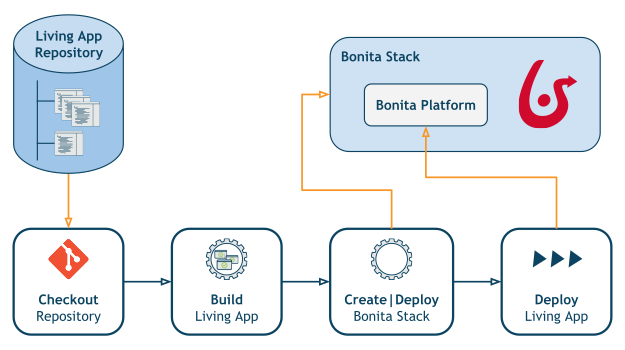
\includegraphics[width=\textwidth,keepaspectratio]{bcd_capabilities.png}
\caption{Fonctionnalités BCD}
\label{fig:bcd_cap}
\end{figure}
